% Basic stuff
\documentclass[a4paper,10pt]{article}
% Uncomment if you use pdfLaTeX
%\usepackage[utf8]{inputenc}
\usepackage[nswissgerman]{babel}

\usepackage{lipsum}

% 3 column landscape layout with fewer margins
\usepackage[landscape, left=0.75cm, top=1cm, right=0.75cm, bottom=1.5cm, footskip=15pt]{geometry}
\usepackage{flowfram}
\ffvadjustfalse
\setlength{\columnsep}{1cm}
\Ncolumn{3}

% define nice looking boxes
\usepackage[most]{tcolorbox}

% a base set, that is then customised
\tcbset {
  base/.style={
    boxrule=0mm,
    leftrule=1mm,
    left=1.75mm,
    arc=0mm, 
    fonttitle=\bfseries, 
    colbacktitle=black!10!white, 
    coltitle=black, 
    toptitle=0.75mm, 
    bottomtitle=0.25mm,
    title={#1}
  }
}

\definecolor{brandblue}{rgb}{0.34, 0.7, 1}
\newtcolorbox{mainbox}[1]{
  colframe=brandblue, 
  base={#1}
}

\newtcolorbox{subbox}[1]{
  colframe=black!20!white,
  base={#1}
}

% Mathematical typesetting & symbols
\usepackage{amsthm, mathtools, amssymb} 
\usepackage{marvosym, wasysym}
\usepackage{derivative}
\allowdisplaybreaks

% Tables
\usepackage{tabularx, multirow}
\usepackage{booktabs}

% Make enumerations more compact
\usepackage{enumitem}
\setitemize{itemsep=0.5pt}
\setenumerate{itemsep=0.75pt}

% To include sketches & PDFs
\usepackage{graphicx}

% For hyperlinks
\usepackage{hyperref}
\hypersetup{
  colorlinks=true
}

% Metadata
\title{Cheatsheet Analysis 2}
\author{Julian Steinmann}
\date{January 2022}

% Math helper stuff
\def\limn{\lim_{n\to \infty}}
\def\limxo{\lim_{x\to 0}}
\def\limxi{\lim_{x\to\infty}}
\def\limxn{\lim_{x\to-\infty}}
\def\sumk{\sum_{k=1}^\infty}
\def\sumn{\sum_{n=0}^\infty}
\def\R{\mathbb{R}}
\def\C{\mathbb{C}}
\def\Q{\mathbb{Q}}
\def\N{\mathbb{N}}
\def\X{\mathcal{X}}
\def\dx{\text{ d}x}

\begin{document}

\maketitle

% Not actually an abstract. We abuse it for licencing
\renewcommand{\abstractname}{License}
\begin{abstract}
  Dieses Dokument ist unter CC BY-SA 4.0 lizenziert. Es darf verbreitet oder verändert werden, solange der Urheber und die Lizenz erhalten bleibt. \\

 \begin{center}
 Der \LaTeX-Quelltext ist verfügbar auf \\ \href{https://github.com/XYQuadrat/eth-cheatsheets}{github.com/XYQuadrat/eth-cheatsheets}.
 \end{center}
\end{abstract}

\section{Differentialgleichungen}
\begin{mainbox}{Definition lineare DGL}
  Eine gewöhnliche lineare Differentialgleichung ist eine Gleichung, welche Ableitungen enthält. Sie hat die Form \[y^{(n)} + a_{n-1} y^{(n-1)} + \cdots + a_0y = b(x)\]
  wo die Koeffizienten \(a_0, \ldots, a_{n-1}\) komplexe Funktionen auf \(I \subset \R\) sind, welche von \(y\) abhängig sein können. Wenn \(b(x) = 0\) gilt, ist die DGL homogen.
\end{mainbox}
Die Menge \(S\) an Lösungen ist ein Subset des Raums der komplexen Funktionen auf \(I\) mit Dimension \(n\). \\
\(S_0\) das Set der Lösungen zu einer homogenen DGL. Für ein \(b(x)\) ist die Menge der Lösungen \(S_b = \{f_h + f_p \mid f_h \in S_0\}\).
\subsubsection*{Lineare DGL erkennen}
\begin{itemize}
  \item keine Koeffizienten vor der höchsten Ableitung
  \item alle Koeffizienten sind stetige Funktionen
  \item keine Produkte von $y$ oder deren Ableitungen
  \item keine Potenzen von $y$ oder deren Ableitungen
  \item keine von $y$ oder deren Ableitungen abhängige Funktionen
\end{itemize}

\subsection{Lineare DGL erster Ordnung}
Wir betrachten DGL der Form \[y' + a(x)y = b(x)\]
\begin{enumerate}
  \item (Homogene Lösung) 
  \begin{align*}
    y' + a(x)y &= 0\\
    \frac{y'}{y} &= -a(x)\\
    \ln(y) &= -A(x)+C\\
    y &= e^{-A(x)+C} = z \cdot e^{-A(x)}\quad z \in \C
  \end{align*}
  \item (partikuläre Lösung) Verwende entweder ``Variation der Konstanten'' oder ``Fundiertes Raten''.
\end{enumerate}
\subsection{Variation der Konstanten}
Sei \(f_p = z(x)e^{-A(x)}\) für eine Funktion \(z: I \to \C\). Wir 


\section{Ableitungen in \(\R^n\)}
\begin{subbox}{Monom}
  Ein Monom vom Grad \(e\) ist
  \begin{align*}
    (x_1, \ldots, x_n) \mapsto x_1^{d_1}\cdot \ldots \cdot x_n^{d_n} \\
    e = d_1 + \ldots + d_n 
  \end{align*}
  \(\to\) ein Polynom, das nur aus einem Glied besteht.
\end{subbox}
\begin{mainbox}{Polynom}
  Ein Polynom mit \(n\) Variablen vom Grad \(d\) ist eine endliche Summe von Monomen mit Grad \(e \le d\).
\end{mainbox}

\subsection{Konvergenz}
\begin{enumerate}
  \item Skalarprodukt: \(\left< x,y\right> = \sum_{i=0} x_i \cdot y_i\)
  \item Euklidische Norm: \(||x|| := \sqrt{x_2^1 + \cdots + x_n^2}\) mit den folgenden Eigenschaften:
  \begin{enumerate}
    \item \(||x|| \ge 0, ||x|| = 0 \iff x = 0\)
    \item \(||\lambda x|| = |\lambda| \cdot ||x||, \forall \lambda \in \R\)
    \item \(||x+y|| \le ||x|| + ||y||\)
    \item \(|\left<x,y\right>| \le ||x|| \cdot ||y||\)
  \end{enumerate}
\end{enumerate}

\begin{mainbox}{Definition Konvergenz}
  Sei \((x_k)_{k \in \mathbb{N}}, x_k \in \R^n\). Die folgenden Definitionen sind für \(\lim_{k\to\infty}x_k = y\) äquivalent:
  \begin{enumerate}
    \item \(\forall \epsilon > 0 \exists N \ge 1\) so dass \(\forall k \ge N \ ||x_k - y|| < \epsilon\).
    \item Für jedes \(i, 1 \le i \le n\) konvergiert die Folge \((x_{k,i})_k\) von reellen Zahlen nach \(y_i\).
    \item Die Folge der reellen Zahlen \(||x_k - y||\) konvergiert nach \(0\).
  \end{enumerate}
\end{mainbox}
\subsection{Stetigkeit}
Sei \(f: \X \subset \R^n \to \R^m\)  und \(x_0 \in \X\). \(f\) ist stetig in \(x_0\), falls eine der folgenden Bedingungen erfüllt ist:
\begin{enumerate}
  \item \(\forall \epsilon > 0 \exists \delta > 0\) so dass \(x \in \X ||x - x_0|| < \delta \implies ||f(x) - f(x_0)|| < \epsilon\).
  \item \(\forall\) Folgen \((x_k)\) in \(X\) mit \(\lim x_k = x_0\) gilt \(\lim f(x_k) = f(\lim x_k)\).
\end{enumerate}
\(f\) ist stetig in \(\X\) falls \(f\) für jeden Punkt \(x_0 \in \X\) stetig ist. Es gilt:
\begin{enumerate}
  \item \(f(x = x_1, \ldots, x_n) \mapsto (f_1(x),\ldots,f_m(x))\) und \(f_i: \R^n \to \R\) stetig \(\iff \forall i = 1, \ldots, m \ f_i\) stetig.
  \item Lineare Funktionen \(x \mapsto Ax\) sind stetig.
  \item Polynome sind stetig.
  \item Summen und Produkte von stetigen Funktionen sind stetig.
  \item Funktionen unterschiedlicher Variablen sind stetig, falls alle Variablen stetig sind.
  \item Verknüpfungen stetiger Funktionen sind stetig.
\end{enumerate}
\begin{mainbox}{Sandwich-Lemma}
  Wenn \(f, g, h: \R^n \to \R\) Funktionen mit \(f(x) < g(x) < h(x) \forall x \in \R^n\) sind, dann gilt
  \[\lim_{x\to a} f(x) = \lim_{x \to a} h(x) = L \implies \lim_{x\to a} g(x) = L\]
\end{mainbox}
\subsection{Eigenschaften von Mengen}
Eine Menge \(\X \subset \R^n \) ist
\begin{itemize}
  \item \textbf{beschränkt}, falls die Menge \(\{ ||x|| \mid x \in \X \}\) in \(\R\) beschränkt ist (d.h. \(\exists R \ge 0, \forall x \in \X: ||x|| \le R\)).
  \item \textbf{abgeschlossen}, falls jede Folge \((x_k)_{k\in \N} \subset \X\), die in \(\R^n\) konvergiert, zu einem Punkt in \(y \in \X\) konvergiert. Dies kann mit einem Ball visualisiert werden. Gegenbeispiele: \(\frac{1}{k}, <\).
  \item \textbf{kompakt}, falls sie beschränkt und abgeschlossen ist.
  \item \textbf{offen}, falls ihr Komplement \(\R^n \setminus \X\) abgeschlossen ist.
  \item \textbf{konvex}, falls \(\forall x, y \in \X: \lambda x + (1 - \lambda)y \in \X\) gilt (die Linie zwischen \(x, y\) ist in \(\X\)).
\end{itemize}
Beispiele:
\begin{itemize}
  \item \((a,b) \subset \R\) ist offen.
  \item \(\left[a,b\right) \subset \R\) ist weder offen noch abgeschlossen.
  \item \(\R^n\) und \(\varnothing\) sind offen.
  \item \((a_1, b_1) \times (a_2,b_2) \subset \R^2\) ist offen.
  \item Urbilder von offenen Mengen sind unter stetigen Abbildungen offen.
\end{itemize}
\begin{subbox}{Bolzano-Weierstrass}
  Jede beschränkte Folge in \(\R^n\) hat eine konvergente Teilfolge.
\end{subbox}
\begin{subbox}{Min-Max-Theorem}
  Sei \(\X \subset \R^n, \X \ne \varnothing\) eine kompakte Menge und \(f: \X \to \R\) eine stetige Funktion. Dann ist \(f\) beschränkt und ein Maximum \(x^+\)/Minimum \(x^-\)existieren, so dass
  \[f(x^+) = \sup_{x\in \X} f(x) \quad f(x^-) = \inf_{x \in \X} f(x)\]
\end{subbox}
\subsection{Partielle Ableitungen}
Um eine partielle Ableitung von \(f: \X \subset \R^n \to \R\) (wobei \(\X\) offen) zu finden, betrachten wir alle Variablen bis auf eine als konstant und leiten nach dieser ab.
\[\pdv{f}{x_{0,j}} = \lim_{h \to 0} \frac{f(x_{0,1}, \ldots, x_{0,j} + h, \ldots, x_{0,n}) - f(x_0)}{h}\]
Für \(f: \R^n \to \R^m, x_0 \in \R^n\) gilt
\begin{align*}
  \pdv{f(x_0)}{x_j} := \begin{pmatrix}
    \pdv*{f_1(x_0)}{x_j}\\
    \vdots\\
    \pdv*{f_m(x_0)}{x_j}\\
  \end{pmatrix}
\end{align*}
Partielle Ableitungen haben folgende Eigenschaften:
\begin{enumerate}
  \item \(\partial_j(f + g) = \partial_j (f) + \partial_j g\)
  \item \(\partial_j(f \cdot g) = \partial_j (f) \cdot g + \partial_j (g) \cdot f\)
  \item \(\partial_j(f / g) = \frac{\partial_j (f) \cdot g - \partial_j (g) \cdot f}{g^2}\) für \(g \ne 0\)
\end{enumerate}
\begin{mainbox}{Jacobi-Matrix}
Sei \(f: \X \subset \R^n \to \R^m\) und \(\X\) eine offene Menge. Die Jacobi-Matrix ist eine Matrix mit \(m\) Zeilen und \(n\) Spalten:
\[J_f = \left( \pdv{f_i}{x_j} \right)_{\substack{1 \leq j \leq n \\ 1 \leq i \leq m}}\]
\end{mainbox}
\begin{mainbox}{Gradient}
  Die Jacobi-Matrix einer Funktion \(f: X \subset \R^n \to \R\) ist ein Spaltenvektor, der mit \(\nabla f\) bezeichnet wird. Die geometrische Interpretation ist ein Vektorfeld, definiert durch \(\nabla f\), welches die Richtung und Magnitude des grössten Wachstums von \(f\) angibt.
\end{mainbox}
\begin{subbox}{Divergenz}
  Die Divergenz einer Funktion \(f\) ist die Spur der Jacobi-Matrix von \(f\). \[\text{div}(f)(x_0) = \text{Tr}(J_f(x_0)) = \sum_{i=0}(J_f)_{i,i}\]
\end{subbox}
\subsection{Differenzierbarkeit}
Sei \(f: \X \subset \R^n \to \R^m, x_0 \in \X\). \(f\) ist differenzierbar an der Stelle \(x_0\), falls eine lineare Abbildung \(L: \R^n \to R^m\) (d.h. eine \(m \times n\)-Matrix \(L\)) existiert, so dass \(\forall x_0 + v \in \X\):
\[f(x_0 + v) = f(x_0) + L(v) + R(x_0,v)\]
wobei für den Fehlerterm \(R\) folgendes gilt: 
\[\lim_{v \to 0} \frac{||R(x_0,v)||}{||v||} = 0\]
Wir schreiben \(df(x_0) = L\). Wenn \(f\) für alle \(x_0 \in \X\) differenzierbar ist, dann ist \(f\) auf \(\X\) differenzierbar. \\
Wenn alle partiellen Ableitungen existieren und stetig sind, dann ist \(f\) differenzierbar.\\
Falls \(f,g\) im Punkt \(x_0 \in \X\) differenzierbar sind, gilt:
\begin{enumerate}
  \item \(f\) ist stetig im Punkt \(x_0\)
  \item \(f\) hat alle partiellen Ableitungen am Punkt \(x_0\) und die Matrix, welche \(df(x_0): x \mapsto Ax\) repräsentiert, ist die Jacobi-Matrix von \(f\) am Punkt \(x_0\), d.h. \(A = J_f(x_0)\)
  \item \(d(f+g)(x_0) = df(x_0) + dg(x_0)\)
  \item Wenn \(m = 1\) ist, dann ist \(f\cdot g\) differenzierbar. Wenn ausserdem \(g \ne 0\) gilt, dann ist es \(f/g\) auch.
  \item Wenn \(f: \X \to Y, g: Y \to \R^m\) beide differenzierbar sind, so gilt \(d(g \circ f)(x_0) = dg(f(x_0)) \circ df(x_0)\). 
  Weiter ist \(J_{g \circ f}(x_0) = J_g(f(x_0)) \cdot J_f(x_0)\).
\end{enumerate}
Die Ableitung einer Funktion ist gegeben durch
\begin{align*}
  f'(x_0) &= \begin{pmatrix}
    f_1'(x_0)\\
    \vdots\\
    f_n'(x_0)
  \end{pmatrix}
\end{align*}
\begin{subbox}{Tagentialraum}
  Der Tangentialraum eines Graphen \(f\) am Punkt \(x_0\) ist gegeben durch \(g(x) = f(x_0) + df(x_0)(x-x_0)\).
\end{subbox}
\subsection{Höhere Ableitungen}
Sei \(\X \subset \R^n\) offen, \(f: \X \mapsto \R^m\). \(f\) ist eine Funktion der Klasse \(C^1\) falls \(f\) auf \(\X\) differenzierbar ist und alles partiellen Ableitungen stetig sind. \\
Allgemein gilt \(f \in \C^k\) für \(k \ge 2\) wenn \(f\) differenzierbar ist und für alle partiellen Ableitungen \(\partial_{x_i} f \in C^{k-1}\) gilt. \\
\(f\) ist glatt oder in \(C^\infty\) falls \(\forall k: f \in C^k \). Alle Polynome sind glatt.

Partielle Ableitungen bis zur Ordnung \(k\) sind kommutativ:
$$\pdv{f}{x_i, x_j} = \pdv{f}{ x_j, x_i}$$

\begin{mainbox}{Hesse-Matrix}
  Die Hesse-Matrix ist eine \(n \times n\) symmetrische Matrix, welche die zweite Ableitung definiert:
  \[\text{Hess}_f(x_0) := \left(\pdv{f(x_0)}{x_i, x_j}\right)_{1\le i,j \le n}\] 
\end{mainbox}
\subsection{Taylorpolynome}
Sei \(k \le 1\) und \(f: \X \mapsto R\) ist eine Funktion der Klasse \(C^k\) auf \(\X\). Sei \(x_0 \in \X\) fix. Das \(k\)-te Taylorpolynom von \(f\) am Punkt \(x_0\) ist das Polynom in \(n\) Variablen vom Grad \(\le k\):
\begin{align*}
  &T_k f(y; x_0) = f(x_0) + \sum_{i=1}^n \partial_i f(x_0) \cdot y_i + \dots \\
  &+ \sum_{m_1 + \cdots + m_n = k} \frac{1}{m_1! \cdots m_n!} \pdv{^k f(x_0) }{x_1^{m_1} \cdots \partial x_n^{m_n}} \cdot y_1^{m_1} \cdots y_n^{m_n}
\end{align*}
Mit folgender Notation kann der Term vereinfacht werden:
\begin{align*}
    m!  &= m_1! \cdots m_n! \\
    |m| &= m_1 + ... + m_n \\
    y^m &= y_1^{m_1} \cdots y_n^{m_n} \\
    \partial_x^m f &= \frac{\partial^{|m|} f}{\partial x_1^{m_1} \cdots \partial x_n^{m_n}}
\end{align*}
Dann ist der obrige Term gleich
\[T_k f(y; x_0) = \sum_{|m| \leq k} \frac{1}{m!}\partial_x^m f(x_0) \cdot y^m\]
Wenn wir \(E_k f(x, x_0)\) wie folgt definieren:
\[f(x) = T_k f(x - x_0, x_0) + E_k f(x, x_0)\]
dann gilt
\[\lim_{x\to x_0} \frac{E_k f(x,x_0)}{||x-x_0||^k} = 0\]

\subsubsection*{Beispiele}
\begin{align*}
  T_1 f(\vec{x}; x_0) &:= f(x_0) + \nabla f(x_0) \cdot (x - x_0) \\
  T_2 f(\vec{x}; x_0) &:= T_1f + \frac{1}{2} \cdot (x - x_0)^\top \cdot \text{Hess}_f(x_0) \cdot (x - x_0)
\end{align*}

\subsection{Definit}
Eine symmetrische Matrix ist
\begin{itemize}
  \item \textbf{positiv definit}, falls alle Eigenwerte positiv sind.
  \item \textbf{negativ definit}, falls alle Eigenwerte negativ sind.
  \item \textbf{indefinit}, falls sowohl positive als negative Eigenwerte existieren.
\end{itemize}
Eigenwerte können mit dem charakteristischen Polynom gefunden werden:
\begin{align*}
  \text{det} \left(
  \begin{pmatrix}
    a & b\\
    c & d
  \end{pmatrix}
  -
  \begin{pmatrix}
    \lambda & 0\\
    0 & \lambda
  \end{pmatrix}
  \right)
  &=
  \text{det}
  \begin{pmatrix}
    a - \lambda & b\\
    c & d - \lambda
  \end{pmatrix}\\
  &\Rightarrow ad - (a + d) \lambda + \lambda^2 - bc = 0
\end{align*}
Für nichtsymmetrische Matrizen müssen wir für jeden Vektor \(v\) testen, ob \(v^\top A v > 0\) (bzw. \(< 0\)) gilt.
\subsubsection*{Determinante in drei Dimensionen}
\begin{align*}
  a \cdot \text{det}
  \begin{pmatrix}
    e & f\\
    h & i
  \end{pmatrix}
  - b \cdot \text{det}
  \begin{pmatrix}
    d & f\\
    g & i
  \end{pmatrix}
  + c \cdot \text{det}
  \begin{pmatrix}
    d & e\\
    g & h
  \end{pmatrix}
\end{align*}
\subsection{Extrema}
\subsubsection*{Lokale Extrema}
Sei \(f: \X \subset \R^n \mapsto \R\) differenzierbar und \(\X\) eine offene Menge. Dann ist \(x_0 \in \X\) ein lokales Maximum (Minimum) falls wir eine Umgebung \(B_r(x_0) = \{x\in \R^n \mid ||x-x_0|| < r \} \subset \X\) finden können, wo gilt:
\[\forall x \in B_r(x_0): f(x) \le (\ge) f(x_0)\]
Wenn \(x_0 \in \X\) ein lokales Extrema ist, dann gilt ausserdem \(\nabla f(x_0) = 0\).

\subsubsection*{Kritische Punkte}
Ein Punkt \(x_0 \in \X\) wo \(\nabla f(x_0) = 0\) gilt ist ein kritischer Punkt. Wenn \(\det(\text{Hess}_f(x_0)) \ne 0\), dann ist \(x_0\) nicht-degeneriert.
\subsubsection*{Sattelpunkt}
Wenn ein kritischer Punkt weder Maximum noch Minimum ist, dann nennen wir ihn Sattelpunkt.

\subsubsection*{Globale Extrema}
Sei \(f: K \mapsto \R\) und \(K\) kompakt, dann existiert ein globales Extrema von \(f\) und es ist entweder ein kritischer Punkt oder am Rand von \(K\). Um ein solches Extrema zu bestimmen, teilen wir \(K\) in sein Inneres \(\X\) und den Rand \(B\) auf. 

Nun bestimmen wir zuerst wie zuvor die kritischen Punkte von \(\X\). Um die Maximas/Minimas von \(B\) zu bestimmen, benötigen wir nur Wissen aus Analysis I (da von der Form \(\R \mapsto \R\)).
\subsubsection*{Testen von kritischen Punkten}
Sei \(f: \X \subseteq \R^n \mapsto \R, \X\) offen und \(f\in C^2\). Sei \(x_0\) ein nicht-degenerierter kritischer Punkt von \(f\). Dann gilt:
\begin{enumerate}
  \item $\text{Hess}_f(x_0)$ pos. def. \(\implies\) $x_0$ ist lokales Minimum.
  \item $\text{Hess}_f(x_0)$ neg. def. \(\implies\) $x_0$ ist lokales Maximum.
  \item $\text{Hess}_f(x_0)$ indefinit \(\implies\) $x_0$ ist Sattelpunkt.
\end{enumerate}
Dies funktioniert nicht, wenn \(x_0\) ein degenerierter kritischer Punkt ist. In einem solchen Fall müssen die Vorzeichen überprüft werden.
\subsubsection*{Kritische Punkte mit Nebenbedingungen}
Wenn wir Minimas/Maximas einer Funktion \(f: \X \mapsto \R\) mit einer Nebenbedingung \(g(x) = 0, g: \X \mapsto \R\) bestimmen wollen, können wir dafür Lagrange-Multiplikatoren verwenden.
\begin{subbox}{Lagrange-Multiplikator}
  Sei \(\X \subset \R^n\) offen und \(f,g: \X \mapsto \R\) Funktionen der Klasse \(C^1\). Wenn \(Y = \{x \in \X \mid g(x) = 0\) ist, dann ist \(x_0 \in Y\) ein lokales Extrema, welches die Nebenbedingung erfüllt, falls 
  \[\exists \delta > 0, f(y) \le (\ge) f(x_0), \quad \forall y \in B_\delta(x_0) \cap Y\]
  gilt. Nun ist entweder \(\nabla g(x_0) = 0\) oder \(\exists \lambda \in \R, \nabla f(x_0) = \lambda \cdot \nabla g(x_0)\), wobei \(\lambda\) dann Lagrange-Multiplikator gennant wird.
\end{subbox}
\section{Integrale in \(R^n\)}











\newpage

\begin{mainbox}{Partielle Integration}
 \vspace{-12pt}
 $$\int f'(x) g(x) \dx = f(x)g(x) - \int f(x) g'(x) \dx$$
\end{mainbox}
\begin{itemize}
 \item Grundsätzlich gilt: Polynome ableiten ($g(x)$), wo das Integral periodisch ist ($\sin, \cos, e^x$,...) integrieren ($f'(x)$)
 \item Teils ist es nötig, mit $1$ zu multiplizieren, um partielle Integration anwenden zu können (z.B. im Fall von $\int \log(x) \dx$)
 \item Muss eventuell mehrmals angewendet werden
\end{itemize}
\begin{mainbox}{Substitution}
 Um $\int_a^b f(g(x)) \dx$ zu berechnen: Ersetze $g(x)$ durch $u$ und integriere $\int_{g(a)}^{g(b)} f(u) \frac{\text{d}u}{g'(x)}$.
\end{mainbox}
\begin{itemize}
 \item $g'(x)$ muss sich irgendwie herauskürzen, sonst nutzlos.
 \item Grenzen substituieren nicht vergessen.
 \item Alternativ kann auch das unbestimmte Integral berechnet werden und dann $u$ wieder durch $x$ substituiert werden.
\end{itemize}

\begin{mainbox}{Partialbruchzerlegung}
 Seien $p(x), q(x)$ zwei Polynome. $\int \frac{p(x)}{q(x)}$ wird wie folgend berechnet:
 \begin{enumerate}
  \item Falls $\deg(p) \ge \deg(q)$, führe eine Polynomdivision durch. Dies führt zum Integral $\int a(x) + \frac{r(x)}{q(x)}$.
  \item Berechne die Nullstellen von $q(x)$.
  \item Pro Nullstelle: Einen Partialbruch erstellen.
  \begin{itemize}[left=0pt]
   \item Einfach, reell: $x_1 \to \frac{A}{x - x_1}$
   \item $n$-fach, reell: $x_1 \to \frac{A_1}{x - x_1} + \ldots + \frac{A_r}{(x-x_1)^r}$ 
   \item Einfach, komplex: $x^2 + px + q \to \frac{Ax + B} {x^2 + px + q}$
   \item $n$-fach, komplex: $x^2 + px + q \to \frac{A_1x+b_1}{x^2+px+q} + \ldots$
  \end{itemize}
  \item Parameter $A_1, \ldots, A_n$ (bzw. $B_1, \ldots, B_n$) bestimmen. ($x$ jeweils gleich Nullstelle setzen, umformen und lösen).

 \end{enumerate}
\end{mainbox}

\section{Trigonometrie}

\subsection{Regeln}

\subsubsection{Doppelwinkel}
\begin{itemize}
 \item $\sin(2\alpha) = 2 \sin(\alpha) \cos(\alpha)$
 \item $\cos(2\alpha) = \cos^2(\alpha) - \sin^2(\alpha) = 1 - 2 \sin^2(\alpha)$
 \item $\tan(2\alpha) = \frac{2\tan(\alpha)}{1 - \tan^2(\alpha)}$
\end{itemize}

\subsubsection{Addition}
\begin{itemize}
 \item $\sin(\alpha + \beta) = \sin(\alpha) \cos(\beta) + \cos(\alpha) \sin(\beta)$
 \item $\cos(\alpha + \beta) = \cos(\alpha) \cos(\beta) - \sin(\alpha) \sin(\beta)$
 \item $\tan(\alpha + \beta) = \frac{\tan(\alpha) + \tan(\beta)}{1 - \tan(\alpha) \tan(\beta)}$
\end{itemize}

\subsubsection{Subtraktion}
\begin{itemize}
 \item $\sin(\alpha - \beta) = \sin(\alpha) \cos(\beta) - \cos(\alpha)\sin(\beta)$
 \item $\cos(\alpha - \beta) = \cos(\alpha) \cos(\beta) + \sin(\alpha)\sin(\beta)$
 \item $\tan(\alpha - \beta) = \frac{\tan(\alpha) - \tan(\beta)}{1+\tan(\alpha) \tan(\beta)}$
\end{itemize}

\subsubsection{Multiplikation}
\begin{itemize}
 \item $\sin(\alpha) \sin(\beta) = -\frac{\cos(\alpha + \beta) - \cos(\alpha - \beta)}{2}$
 \item $\cos(\alpha) \cos(\beta) =  \frac{\cos(\alpha + \beta) + \cos(\alpha - \beta)}{2}$
 \item $\sin(\alpha) \cos(\beta) =  \frac{\sin(\alpha + \beta) + \sin(\alpha - \beta)}{2}$
\end{itemize}

\subsubsection{Potenzen}
\begin{itemize}
 \item $\sin^2(\alpha) = \frac{1}{2}(1-\cos(2\alpha))$
 \item $\cos^2(\alpha) = \frac{1}{2}(1+\cos(2\alpha))$
 \item $\tan^2(\alpha) = \frac{1-\cos(2\alpha)}{1+\cos(2\alpha)}$
\end{itemize}

\subsubsection{Diverse}

\begin{itemize}
 \item $\sin^2(\alpha) + \cos^2(\alpha) = 1$
 \item $\cosh^2(\alpha) - \sinh^2(\alpha) = 1$
 \item $\sin(z) = \frac{e^{iz} - e^{-iz}}{2}$ und $\cos(z) = \frac{e^{iz} + e^{-iz}}{2}$
\end{itemize}

% start larger spacing in tables
\begingroup
\renewcommand*{\arraystretch}{2}

\begin{mainbox}{Wichtige Werte}
  \begin{center} 
    \begin{tabular}{c|cccccc}
      deg & 0° & 30° & 45° & 60° & 90° & 180° \\
      \midrule
      rad & 0 & $\frac{\pi}{6}$ & $\frac{\pi}{4}$ & $\frac{\pi}{3}$ & $\frac{\pi}{2}$ & $\pi$ \\
      cos & 1 & $\frac{\sqrt{3}}{2}$ & $\frac{\sqrt{2}}{2}$ & $\frac{1}{2}$ & 0 & -1 \\
      sin & 0 & $\frac{1}{2}$ & $\frac{\sqrt{2}}{2}$ & $\frac{\sqrt{3}}{2}$ & 1 & 0 \\
      tan & 0 & $\frac{1}{\sqrt{3}}$ & 1 & $\sqrt{3}$ & $+\infty$ & 0 \\
    \end{tabular}
  \end{center}
\end{mainbox}

\begin{center}
  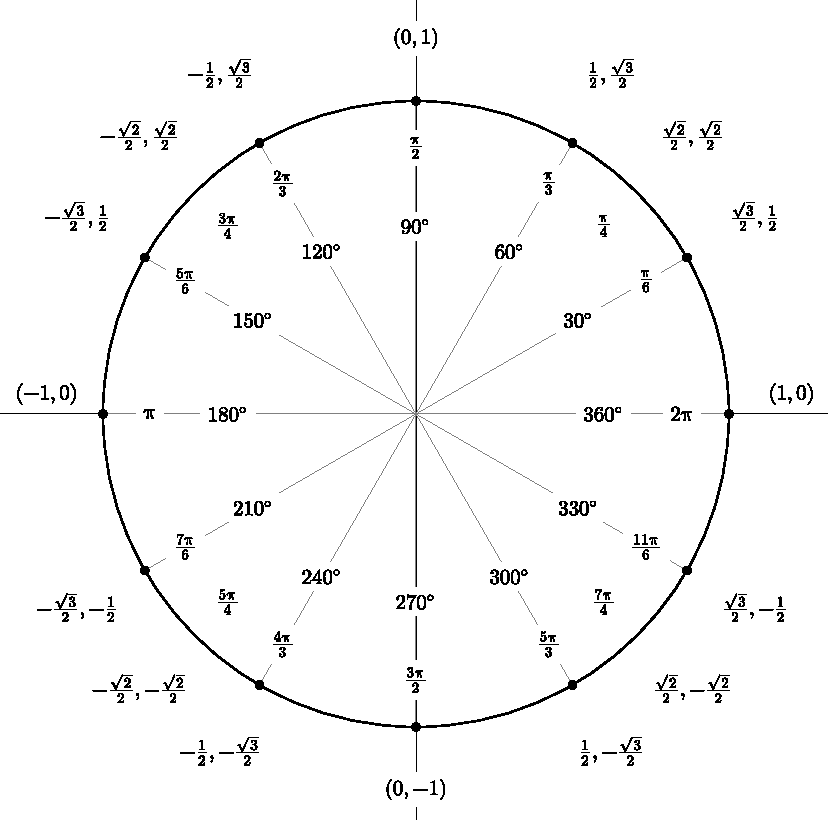
\includegraphics[width=\linewidth]{include_degrees_circle.pdf}
  
\end{center}

\section{Tabellen}
\subsection{Ableitungen}
\begin{center}
  % the c>{\centering\arraybackslash}X is a workaround to have a column fill up all space and still be centered
  \begin{tabularx}{\linewidth}{c>{\centering\arraybackslash}Xc}
    \toprule
    $\mathbf{F(x)}$ & $\mathbf{f(x)}$ & $\mathbf{f'(x)}$ \\
    \midrule
    $\frac{x^{-a+1}}{-a+1}$ & $\frac{1}{x^a}$ & $\frac{a}{x^{a+1}}$ \\
    $\frac{x^{a+1}}{a+1}$ & $x^a \ (a \ne 1)$ & $a \cdot x^{a-1}$ \\
    $\frac{1}{k \ln(a)}a^{kx}$ & $a^{kx}$ & $ka^{kx} \ln(a)$ \\
    $\ln |x|$ & $\frac{1}{x}$ & $-\frac{1}{x^2}$ \\
    $\frac{2}{3}x^{3/2}$ & $\sqrt{x}$ & $\frac{1}{2\sqrt{x}}$\\
    $-\cos(x)$ & $\sin(x)$ & $\cos(x)$ \\
    $\sin(x)$ & $\cos(x)$ & $-\sin(x)$ \\
    $\frac{1}{2}(x-\frac{1}{2}\sin(2x))$ & $\sin^2(x)$ & $2 \sin(x)\cos(x)$ \\
    $\frac{1}{2}(x + \frac{1}{2}\sin(2x))$ & $\cos^2(x)$ & $-2\sin(x)\cos(x)$ \\
    \multirow{2}*{$-\ln|\cos(x)|$} & \multirow{2}*{$\tan(x)$} & $\frac{1}{\cos^2(x)}$  \\
    & & $1 + \tan^2(x)$ \\
    $\cosh(x)$ & $\sinh(x)$ & $\cosh(x)$ \\
    $\log(\cosh(x))$ & $\tanh(x)$ & $\frac{1}{\cosh^2(x)}$ \\
    $\ln | \sin(x)|$ & $\cot(x)$ & $-\frac{1}{\sin^2(x)}$ \\
    $\frac{1}{c} \cdot e^{cx}$ & $e^{cx}$ & $c \cdot e^{cx}$ \\
    $x(\ln |x| - 1)$ & $\ln |x|$ & $\frac{1}{x}$ \\
    $\frac{1}{2}(\ln(x))^2$ & $\frac{\ln(x)}{x}$ & $\frac{1 - \ln(x)}{x^2}$ \\
    $\frac{x}{\ln(a)} (\ln|x| -1)$ & $\log_a |x|$ & $\frac{1}{\ln(a)x}$ \\
    \bottomrule
  \end{tabularx}
\end{center}
\subsection{Weitere Ableitungen}
\begin{center}
  \begin{tabularx}{\linewidth}{>{\centering\arraybackslash}X>{\centering\arraybackslash}X}
    \toprule
    $\mathbf{F(x)}$ & $\mathbf{f(x)}$ \\
    \midrule
    $\arcsin(x)$ & $\frac{1}{\sqrt{1 - x^2}}$ \\
    $\arccos(x)$ & $\frac{-1}{\sqrt{1 - x^2}}$ \\
    $\arctan(x)$ & $\frac{1}{1 + x^2}$ \\ 
    $x^x \ (x > 0)$ & $x^x \cdot (1 + \ln x)$ \\
    \bottomrule
  \end{tabularx}
\end{center}
\subsection{Integrale}
\begin{center}
  \begin{tabularx}{\linewidth}{>{\centering\arraybackslash}X>{\centering\arraybackslash}X}
    \toprule
    $\mathbf{f(x)}$ & $\mathbf{F(x)}$ \\
    \midrule
    $\int f'(x) f(x) \dx$ & $\frac{1}{2}(f(x))^2$ \\
    $\int \frac{f'(x)}{f(x)} \dx$ & $\ln|f(x)|$ \\
    $\int_{-\infty}^\infty e^{-x^2} \dx$ & $\sqrt{\pi}$ \\
    $\int (ax+b)^n \dx$ & $\frac{1}{a(n+1)}(ax+b)^{n+1}$ \\
    $\int x(ax+b)^n \dx$ & $\frac{(ax+b)^{n+2}}{(n+2)a^2} - \frac{b(ax+b)^{n+1}}{(n+1)a^2}$ \\
    $\int (ax^p+b)^n x^{p-1} \dx$ & $\frac{(ax^p+b)^{n+1}}{ap(n+1)}$ \\
    $\int (ax^p + b)^{-1} x^{p-1} \dx$ & $\frac{1}{ap} \ln |ax^p + b|$ \\
    $\int \frac{ax+b}{cx+d} \dx$ & $\frac{ax}{c} - \frac{ad-bc}{c^2} \ln |cx +d|$ \\
    $\int \frac{1}{x^2+a^2} \dx$ & $\frac{1}{a} \arctan \frac{x}{a}$ \\
    $\int \frac{1}{x^2 - a^2} \dx$ & $\frac{1}{2a} \ln\left| \frac{x-a}{x+a} \right|$ \\
    $\int \sqrt{a^2+x^2} \dx $ & $\frac{x}{2}f(x) + \frac{a^2}{2}\ln(x+f(x))$ \\
    \bottomrule
  \end{tabularx}
\end{center}

% end of larger array spacing
\endgroup

\end{document}
